\chapter{Beschreibung des Programmablaufs}
Über einen konfigurierbaren Crawler können HTML-Inhalte von Webseiten bis zu einer bestimmten Tiefe
aus dem Netz in ein Archiv geladen werden. Da dies parallelisiert erfolgen soll,
müssen die Daten nach dem Herunterladen von temporären Verzeichnissen in das gemeinsame
Archivverzeichnis synchronisiert kopiert werden. Der extrahierte Pfad der HTML-Dateien wird
dabei auf das Archiv abgebildet, wobei jede HTML-Datei in einen eigenen Archivordner verschoben wird. \\
Beim Crawlvorgang werden zusätzlich Metadaten der HTML-Seiten erstellt. 
Diese werden in einer Datenbank und als XML-Datei im jeweiligen HTML-Ordner gespeichert.
Die Datenbank soll dabei wieder aus den XML-daten rekonstruierbar sein. \\
Über eine Java-Schnittstelle kann anschließend wieder auf die Daten zugegriffen werden.
Dabei sollen neben dem Auslesen von vorhandenen Dateien auch neue Dateien den Archivordnern hinzugefügt werden können.
Ebenso sollen die oben genannten XML-Daten um neue Nodes erweiterbar sein.

\chapter{Datenmodell der Metadaten}
Für vereinfachte Such- und Sortieraufgaben wird bereits ein vereinfachtes Datenmodell festgelegt, welches
später auf Datenbank und XML-Daten umgesetzt werden soll: \\\\
\begin{tabular}{|l|l|}
	\hline
	Name & Datentyp \\
	\hline
	URL & String \\
	Dateipfad des Archivordners im Archiv & String \\
	Hashsumme über den Content &  String \\
	Datum der letzten Änderung & TimeStamp oder Integer \\
	Commit Tag der Versionsverwaltung & String \\
	\hline
\end{tabular}

\chapter{Programmteile}

\section{Crawlermodul}
Die Steuerung des bzw. der Crawler erfolgt über eine Config-Datei. 
Optional kann das Modul mittels Kommandozeileninterface mit Parametern gestartet werden.
Es können folgende Parameter eingestellt werden:
\begin{itemize}
	\item Tiefe bis zu der Links gefolgt werden soll
	\item Zeitintervalle der Crawlvorgänge
	\item maximale Anzahl der gleichzeitig gestarteten Crawlerinstanzen
	\item Domains, also die Startpunkte für die Crawler, pro Domain wird dann ein Crawler gestartet,
		bis die Obergrenze erreicht wurde.
\end{itemize}

\subsection{Crawlvorgang} \label{l:spez:crawler}
Für die Crawlerinstanzen wird ein externes Tool verwendet (z.B. wget).
Jede gestartete Instanz kopiert den Inhalt der Seite in je ein temporäres Verzeichnis.
Dabei wird die online vorhandene URL-Pfadstruktur der HTML-Dateien auf das Dateisystem abgebildet.
Je Domain wird dadurch ein Hauptverzeichnis erzeugt. \\
Nach diesem Vorgang werden die temp-Ordner bereinigt (z.B. leere Ordner entfernt)
und die HTML-Dateien in ein Archiv-Ordner gleichen Namens kopiert.
Nun werden die Metadateien im XML-Format extrahiert und im o.g. Ordner gespeichert.
Zuletzt werden die so vorbereiteten tmp-Ordner in das vorhandene Archiv hineinsynchronisiert (z.B. mit rsync). 
Dabei wird jeder Domainordner über ein Dateimutex gelockt, um
gleichzeitiges Schreiben zu verhindern. \\
Zum Abschluss werden die Änderungen den Versionsverwaltungen der Domainordner mit einem Commit bestätigt.
Während oder nach dem Synchronisationsvorgang wird ein Datenbank-Dump für die neuen oder geänderten Daten
zur Aktualisierung der Datenbank erstellt.

\section{Archiv}
Das Verzeichnis ist in einzelne Domainordner getrennt. Jeder Domainordner wird über ein Versionsverwaltung
(z.B. git) versioniert. Damit ist das Wiederherstellen älterer Versionen grundsätzlich möglich,
wobei diese aber manuell über die git-Schnittstellen abgerufen werden müssen.
Bei Schreibvorgängen muss ähnlich wie unter \ref{l:spez:crawler} beschrieben, 
die Daten gegen konkurrierende Dateizugriffe gesichert werden.
\paragraph{Dateisystem:} Beim darunterliegenden Dateisystem wird von einem Linuxsystem ausgegangen.
\paragraph{Komprimierung:} Eine explizite Dateikomprimierung wird erstmal nicht vorgesehen, ist aber 
	zum Teil schon durch die Versionsverwaltung gegeben.

\section{Programmierschnittstelle - Java-Client}
Über diesen Client können vorbereitete Sql-Statements an einen Java-Server geschickt werden. Als return-Wert
wird eine Liste von Metadatenobjekten zurückgegeben.
Über diese Metadatenobjekte kann man sich nun über eine gesonderte Anfrage die vorhandenen Archivordner aus dem Archiv nachladen.
Auch eine Erweiterung der XML-Dateien um neue Tags bzw. die Abfrage von Tags soll über die 
Metadatenobjekte möglich sein.

\section{XML-Metadaten}
Die XML-Datei enthält grundsätzliche Metainformationen über eine archivierte HTML-Datei.
Die XML-Datei soll auch nachträglich über eine Programmierschnittstelle um weitere XML-tags erweiterbar sein.
Umgesetzt wird dies über die oben genannten Objekte der Java-Metadatenklasse, 
der bei Übergabe eines Namens an eine get-Methode ein passender XML-Node herausgesucht wird.
Mittels einer set-Methode, die Namen und Inhalt des Tags als Parameter erhält, können neue Tags hinzugefügt werden. 

\section{Datenbank}
Die Datenbank dient zur Speicherung der grundlegenden Metadaten und soll schnelle Suchanfragen zu ermöglichen.
Die Datenband muss beim Fertigstellen des Crawlvorgangs auf den neuesten Stand gebracht werden.
Sollte die Datenbank beschädigt oder geändert werden, dann soll diese wieder aus den
XML-Metadaten rekonstruiert werden können.
Aus diesem Grund wird erstmal von einer sqlite-Datenbank ausgegangen, 
da diese relativ einfach als Datei erstellt und wieder gelöscht werden kann. 

\section{Anmerkung: Programmiersprachen}
Für die systemnahen Programmteile, wie die Steuerung der Crawler wird die Sprache Python in der Version 2 verwendet,
da hier bereits gute Libraries für den Zugriff auf das Dateisystem und die Versionsverwaltung vorhanden sind.
Die mehr objektorientierten Teile und Schnittstellen nach außen werden in Java umgesetzt.
 
% Diagramm

\begin{figure}
	\centering
	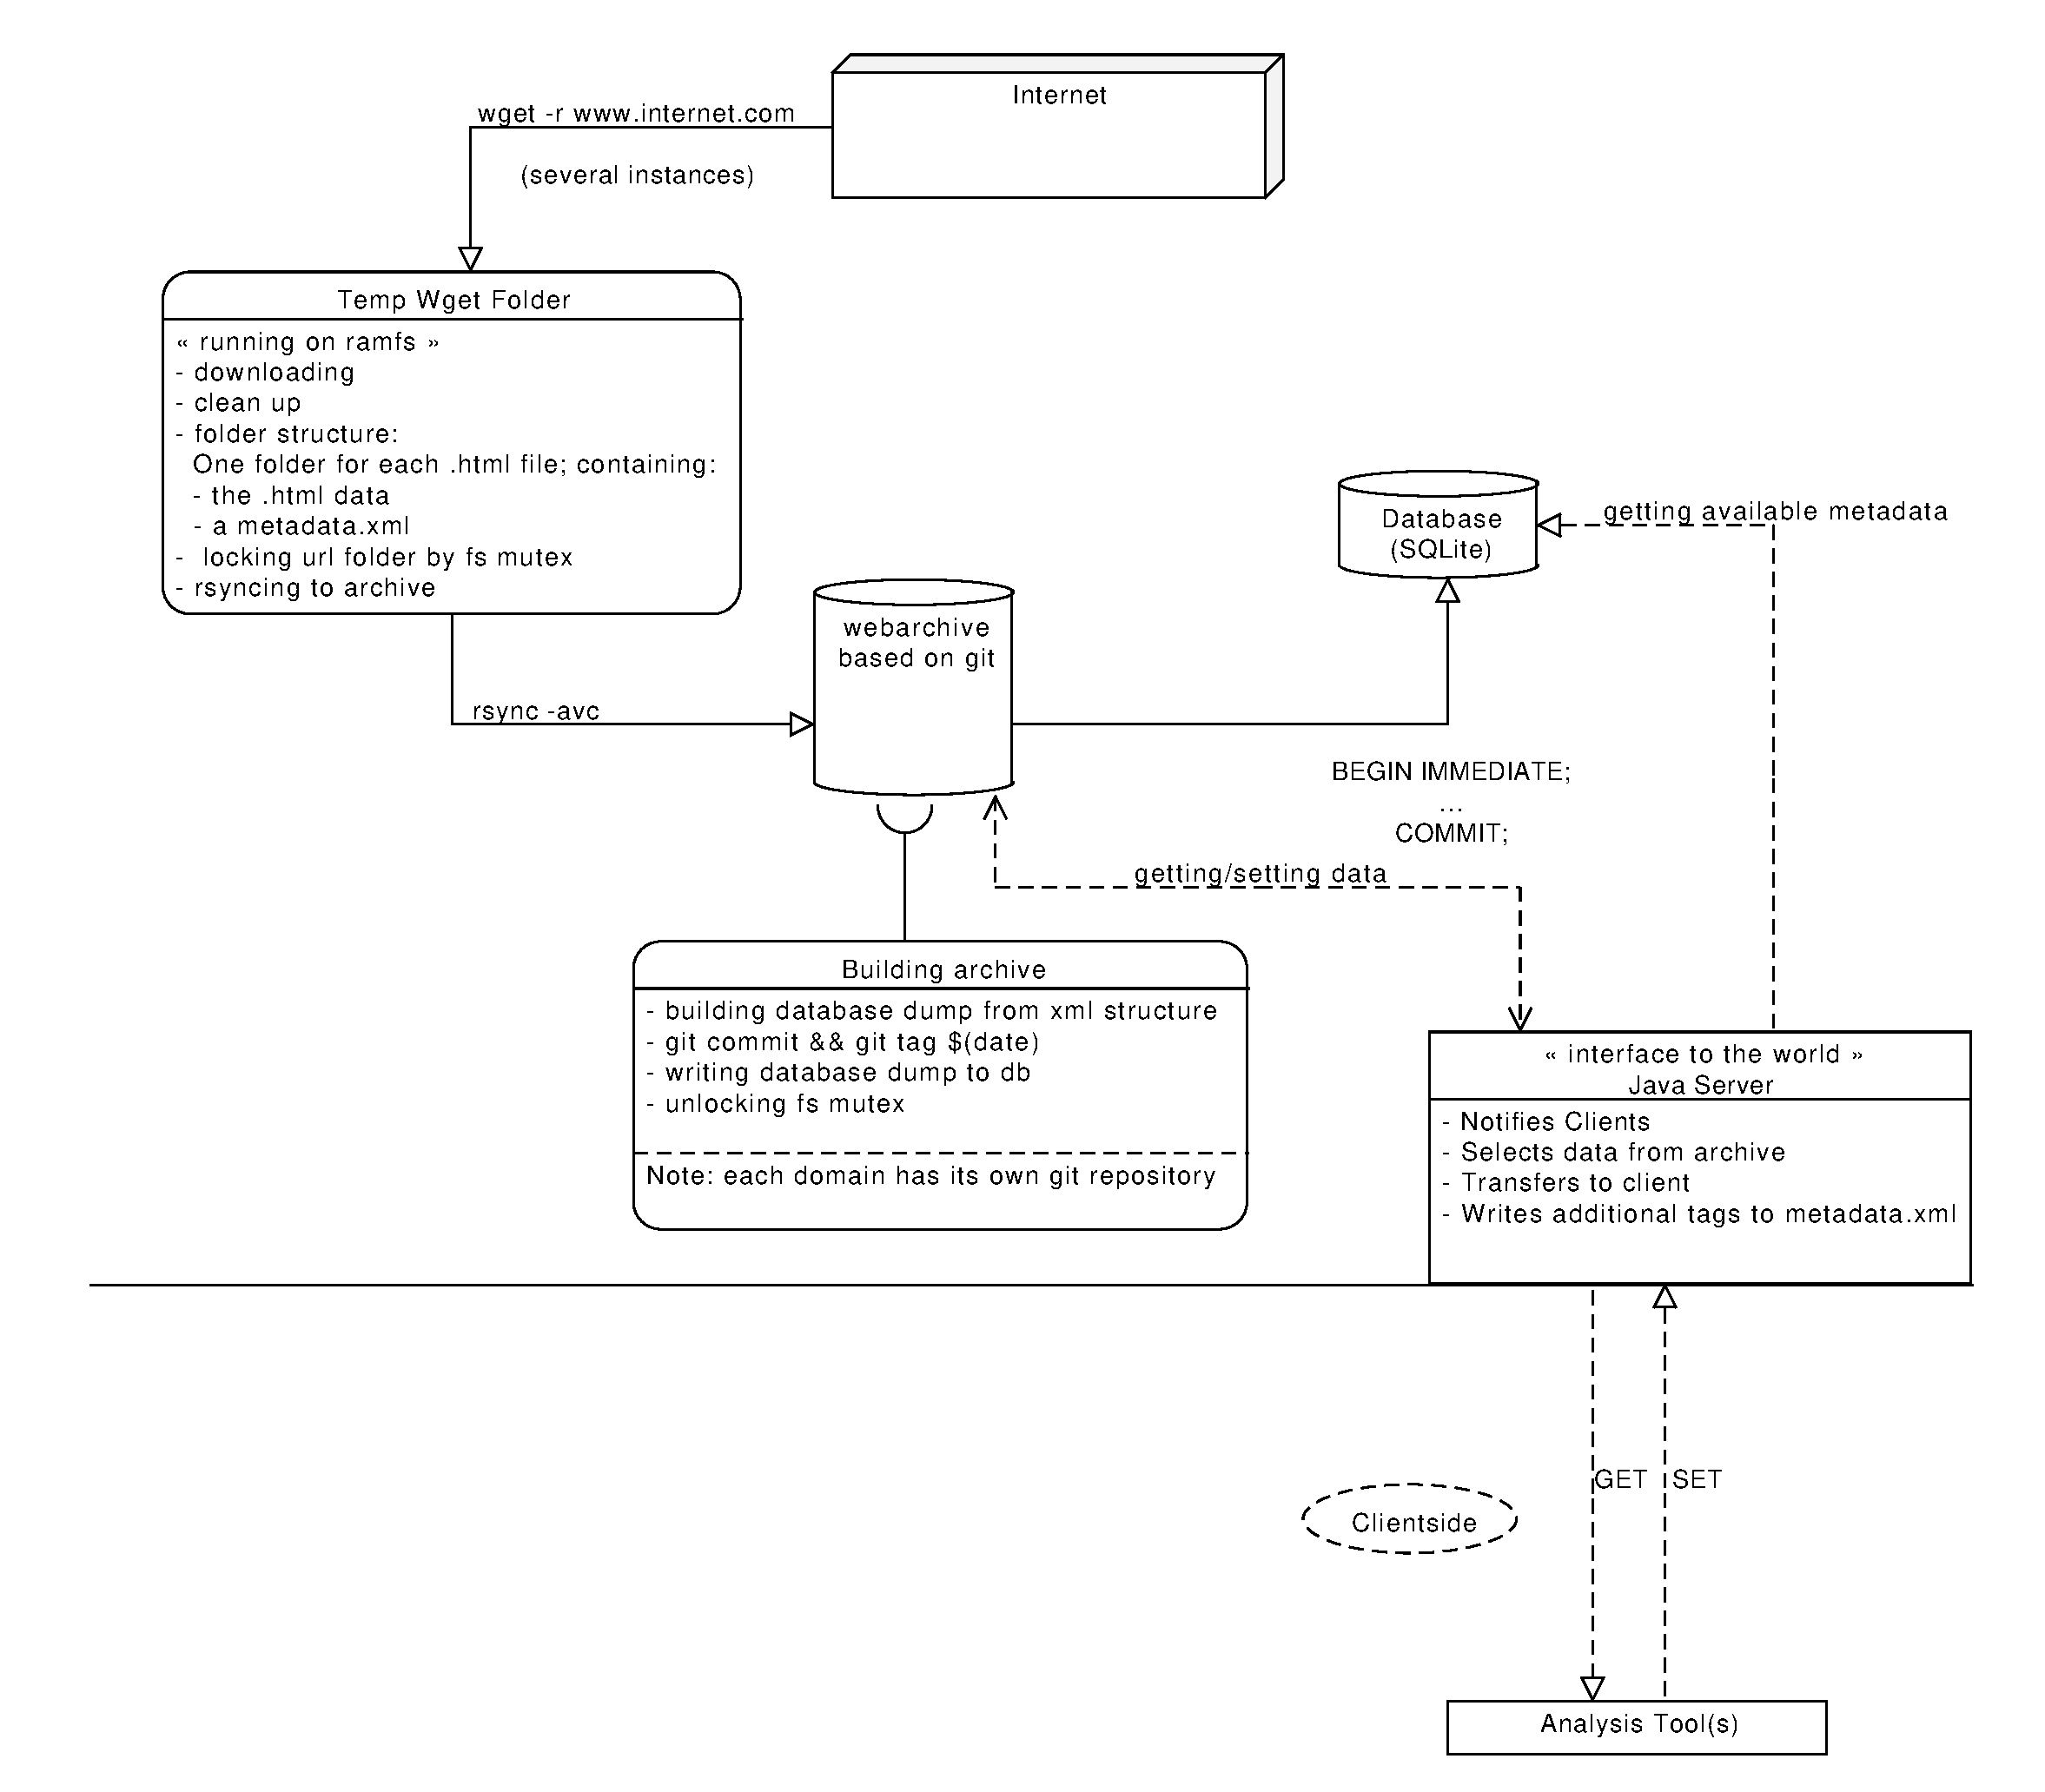
\includegraphics[width=\textwidth]{spezi/webarchiv_design.pdf}
	\caption{Diagramm: Grundlegendes Design}
\end{figure}
 
